More details will be given in the workflow of GASAL2 and its distinctive features. Finally, we will outline a list of characteristics we need for GASAL2 to be integrated in BWA-MEM.


\subsection{Typical workflow of GASAL2}

We will now describe the workflow usually followed when using GASAL2. Figure~\ref{fig:dataflow} shows this flow in a graph. This flow can be instantiated multiple times from each CPU threads.

The first step is to fill the parameters used for alignment: match and mismatch scores, maximum number of sequences and maximum sizes. Then the GPU and host storages are initialised with this given size. Data sizes are specified in advance, so the initialisation takes an important amount of VRAM.

Then, the first available stream is selected. It is filled up with the query and target sequences and their metadata (lengths, offsets, operations for reverse/complementing if needed). Then it launches the non-blocking call for the GPU memory copies and kernel launches. These particular calls are represented in the yellow block. Note that no direct array links functions from outside the block to the inside. This is meant to show that the CPU, once making the non-blocking calls, directly jumps to the next blue box in the graph, and performs the next tasks.

Finally, if a stream has finished, its results are retrieved. The streams allows for full CPU-GPU overlap execution, giving significant speed-up, as we will see later on.

\begin{figure}[p]
	\centering
	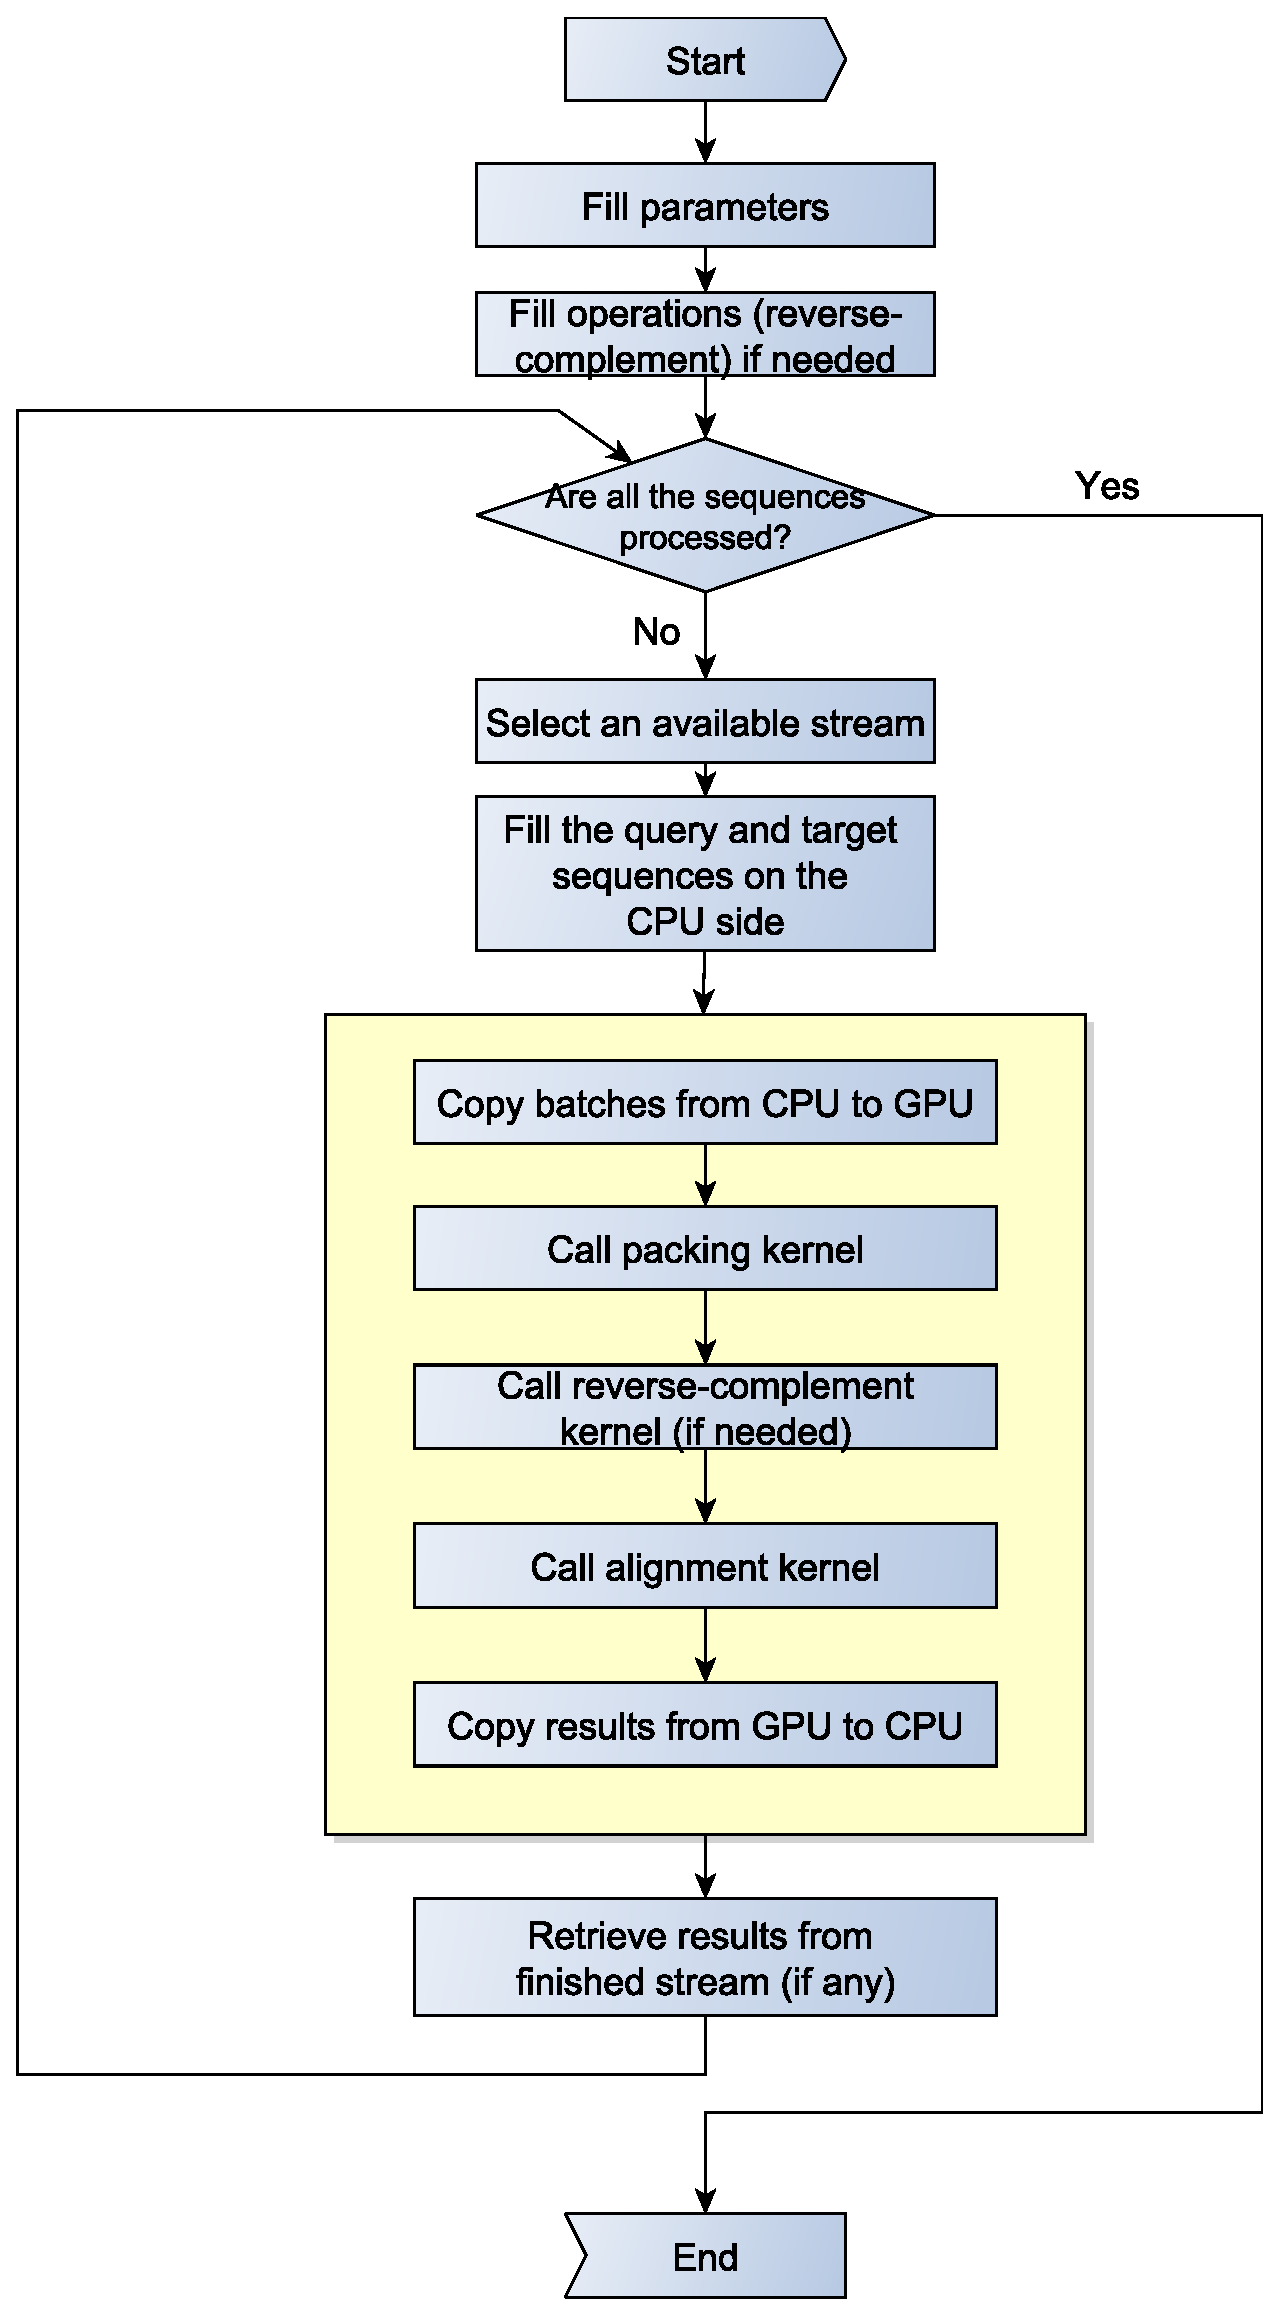
\includegraphics[width=0.85\linewidth]{dataflow}
	\caption{GASAL2 typical workflow}
	\label{fig:dataflow}
\end{figure}


%\begin{algorithm}
%	\caption{GASAL2 workflow}
%	\label{euclid}
%	\begin{algorithmic}[1] % The number tells where the line numbering should start
%		\Procedure{Align a batch of sequences}{} \Comment{}
%		
%		\While {not all sequences are aligned}
%			\State Select the first available stream
%			
%			\For {Each pair of sequences}
%				\State Copy the target sequence to the host buffer
%				\State Copy the query sequence to the host buffer
%				\State Store the length to the host array
%				\If {There is a reverse/complement operation to run}
%					\State Store the operation to the host array
%				\EndIf
%			\EndFor
%			
%			\State Select the first finished stream if any
%			
%		
%		\EndWhile
%		
%		\EndProcedure
%	\end{algorithmic}
%	\begin{algorithmic}[1] % The number tells where the line numbering should start
%	\Procedure{Launch batch alignment}{} \Comment{}
%	
%		\State Launch the copy from host to device
%		\State Launch the data packing kernel on GPU
%		\State Launch the reverse/complement kernel on GPU
%		\State Launch the alignment kernel on GPU
%		
%	\EndProcedure
%	\end{algorithmic}
%
%\end{algorithm}

An important feature of GASAL2 is that it packs and compresses the sequences on GPU to accelerate its handling in the alignment kernel. There are 5 different bases possible: A, T, C, G and the unknown base N. This means that a minimum of 3 bits is needed to encore 5 different values. The bases are then stored in 32-bits words. The goal is to allow the alignment kernel to fetch a pack of bases from the VRAM, put them in the cache, and then perform operations on the cached bases. This cache memory on a GPU is extremely small (for example, each SM can give its threads an access to 48KB of L1 cache for the GPU in our test machine~\cite{nvidia:keplerarch}), but very fast and close to the computing resources.
However, using 3 bits would mean needing a lot of bitwise operations to uncompress the data, since it would not align easily with 32-bits words. This is why the decision has been made to use 4 bits to encode the base value, hence, 8 bases are stored in each 32-bit word. This way, the kernel fetches two 32 bits words (one for query, one for target) and can easily uncompress the 8 bases stored. The dynamic programming matrix is then computed in tiles of 8 $\times$ 8 cells.


\subsection{Characteristics of GASAL2 launches}

The kernel launch has adaptable parameters to tune it for a given data set, number of CPU threads and number of GPU threads, depending on the hardware at hand. GASAL2 in its current state, has up to three different types of kernels:

\begin{itemize}
	\item the packing kernel
	\item the reverse/complement kernel, if needed
	\item the alignment kernel (be it local, global, or else)
\end{itemize}

The packing and the reverse/complement kernels are very fast due to having very few computation, and take almost no time to complete compared to the alignment kernel. With various data sets, it has been measured that the packing kernel takes at most 0.6\% of the kernels run times, and the reverse/complement kernel takes at most 4\% of the kernels run times when all sequences must be both reversed and complemented, and data transfer time take at most 4\% of the total time. Note that these times are given here as a rough estimate to show the importance of some tasks compared to others, and that precise measurements are presented on Chapter~\ref{chap:measurements}. As expected, the large majority of the time is taken by the alignment kernel.

The alignment kernel has a variable GPU occupation depending on the data processed. On our test machine, with a single CPU thread, the SM utilisation oscillates between 3\% and 10\%. Even though it seems a very low occupation, it is not a major problem since the kernels are compute bound and higher occupancy does not necessarily increase the performance.
%% http://developer.download.nvidia.com/compute/DCGM/docs/nvidia-smi-367.38.pdf


\subsection{Extension kernel behaviour}
\label{sec:seedonly}
The aim of this project is to integrate GASAL2 in BWA-MEM to perform the extension part on GPU. To do so, we need to reproduce the behaviour of the extension function of BWA-MEM to replicate it in GASAL2.

The original extension function has a BLAST-like seed-extension behaviour. It starts from a pair of target and query sequences and knowing the position of the beginning of the seed, its length, and its score, it proceeds as follows:
\begin{itemize}
	\item it isolates the left part of both sequences, and reverse them.
	\item it computes a local alignment with the beginning score equal to the seed score. The end position of this alignment is equal to the beginning of the alignment of the two sequences (the alignment progresses from right to left, since the left parts have been reversed)
	\item it then isolates the right part of both sequences,
	\item it computes a local alignment with the start score equal to the left score previously computed (which includes the seed score).
\end{itemize}

In our case, this approach is unpractical because one would like to compute both sides in parallel to maximise GPU usage. In this fashion, we do not have other choices than making both extensions (left and right) start with a score equal to the seed score, which could make a small difference in the final result. We expected this error between the regular BLAST-like computation and our slightly different approach to be small enough to consider this approach valid. We effectively measured it after implementation, with results shown in Chapter~\ref{chap:measurements} and we reached the conclusion that the difference was effectively very small and that calculating both sides at the same time only using the seed score is an acceptable way to solve this problem. We call that paradigm the "seed-only" method.

Another problem comes from the rigidity of GASAL2 memory scheme. Originally, GASAL2 was not able to scale in memory and adapt if some sequences were longer than expected, resulting in a crash of the program. This is particularly problematic when integrating it in BWA-MEM, because the number of seeds is unknown in advance, so each batch in GASAL2 need to have a variable size; plus, left and right parts of the target and query sequences have an unpredictable length. An extensible data structure should be implemented to tackle this issue with minimum overhead.


